\documentclass[11pt]{article}
%\usepackage{psfig}
\usepackage{latexsym}
\usepackage{amsfonts}
\usepackage{hyperref}
\usepackage{url}
\usepackage{listings}
% to use hyperlinks in References section
\hypersetup{urlbordercolor={1 1 1}}
\usepackage{graphicx}
\usepackage{listings}	

%define colors
\usepackage{xcolor} 	
\definecolor{dkgreen}{rgb}{0,0.6,0}
\definecolor{gray}{rgb}{0.5,0.5,0.5}
\definecolor{mauve}{rgb}{0.58,0,0.82}
\usepackage{graphicx}
\usepackage{hyperref}
\hypersetup{urlbordercolor={1 1 1}}
\DeclareGraphicsExtensions{.pdf,.jpg,.png,.eps}
\setlength{\textheight}{8.5in}
\setlength{\textwidth}{6.0in}
\setlength{\headheight}{0in}
\addtolength{\topmargin}{-.5in}
\addtolength{\oddsidemargin}{-.5in}


\newenvironment{cvl}{\begin{list}{$\bullet$}{
\setlength{\leftmargin}{0.3in} \setlength{\labelsep}{0.07in}
\setlength{\labelwidth}{0.17in} \setlength{\rightmargin}{0.0in}
\setlength{\topsep}{0.000in} \setlength{\partopsep}{0.000in}
\setlength{\parskip}{0.000in} \setlength{\parsep}{0.005in}
\setlength{\itemsep}{0.005in}}}{\end{list}}

\DeclareGraphicsExtensions{.pdf,.jpg,.png,.eps}
\usepackage[T1]{fontenc}	%special characters copy-able

\usepackage{times}
\usepackage{enumerate}

%--------------
%% Modified by Zhiqiang Lin
%% 01/18/2012
%%
%% Template file was from http://www.cs.umd.edu/~jkatz
%%
%% preamble.tex
%% this should be included with a command like
%% %--------------
%% Modified by Zhiqiang Lin
%% 01/18/2012
%%
%% Template file was from http://www.cs.umd.edu/~jkatz
%%
%% preamble.tex
%% this should be included with a command like
%% %--------------
%% Modified by Zhiqiang Lin
%% 01/18/2012
%%
%% Template file was from http://www.cs.umd.edu/~jkatz
%%
%% preamble.tex
%% this should be included with a command like
%% \input{preamble.tex}
%% \lecture{``lecture number''}{``date''}{``name of professor''}{``name
%%  of student''}

\hbadness=10000
\vbadness=10000

\newcommand{\handout}[5]{
   \renewcommand{\thepage}{#1-\arabic{page}}
   \noindent
   \begin{center}
   \framebox{
      \vbox{
    \hbox to 5.78in { {\bf CSE 5473 --- Network Security} 
     	 \hfill #2 }
       \vspace{4mm}
       \hbox to 5.78in { {\Large \hfill #5  \hfill} }
       \vspace{2mm}
       \hbox to 5.78in { {\it #3 \hfill #4} }
      }
   }
   \end{center}
   \vspace*{4mm}
}

\newcommand{\lecture}[4]{\handout{#1}{#2}{#3}{#4}{#1}}
%\newcommand{\lecture}[4]{\handout{#1}{#2}{Lecturer: #3}{Scribe(s): #4}{Lecture #1}}

\def\epsilon{\varepsilon}
\def\phi{\varphi}
\def\bool{\{0,1\}}
\def\poly{{\sf poly}}
\def\cross{\times}

\newcommand{\xor}{\oplus}
\newcommand{\Xor}{\bigoplus}
\newcommand{\ceil}[1]{\left\lceil {#1} \right\rceil}
\newcommand{\floor}[1]{\left\lfloor #1 \right\rfloor}
\newcommand{\ignore}[1]{}
\newcommand{\integers}[1]{{\mathbb Z}_{#1}}
\newcommand{\bydef}{\stackrel{\rm def}{=}}
\newcommand{\isequal}{\stackrel{\rm ?}{=}}
\newcommand{\compeq}{\stackrel{\rm c}{\equiv}} % computationally indistinguishable

\newcommand{\qed}{\hspace*{\fill}\rule{7pt}{7pt}}
\newenvironment{proof_sketch}{\noindent{\bf Sketch of Proof} (Informal)\hspace*{1em}}{\qed\medskip}
\newenvironment{proof}{\noindent{\bf Proof}\hspace*{1em}}{\qed\medskip}
\newenvironment{proofof}[1]{\noindent{\bf Proof} of #1:\hspace*{1em}}{\qed\medskip}
%\newenvironment{claim}{\noindent{\bf Claim}\hspace*{1em}\begin{em}}{\end{em}\medskip}
\newcounter{defcounter}
\setcounter{defcounter}{1}
\newenvironment{definition}{\medskip\noindent{\bf Definition \thedefcounter}}{\hspace*{\fill}$\diamondsuit$\stepcounter{defcounter}\medskip}
\newtheorem{theorem}{Theorem}
\newtheorem{corollary}[theorem]{Corollary}
\newtheorem{lemma}[theorem]{Lemma}
\newtheorem{claim}[theorem]{Claim}
\newtheorem{fact}[theorem]{Fact}
\newtheorem{conjecture}[theorem]{Conjecture}
\newenvironment{assumption}{\noindent{\bf Assumption}\hspace*{1em}\begin{em}}{\end{em}\medskip}
\newenvironment{remark}{\noindent{\bf Remark}\hspace*{1em}}{\bigskip}

\ignore{
\newcommand{\FOR}{{\bf for}}
\newcommand{\TO}{{\bf to}}
\newcommand{\DO}{{\bf do}}
\newcommand{\WHILE}{{\bf while}}
\newcommand{\AND}{{\bf and}}
\newcommand{\IF}{{\bf if}}
\newcommand{\THEN}{{\bf then}}
\newcommand{\ELSE}{{\bf else}}

%%% You probably will not need to use the commands listed below

\makeatletter
\def\fnum@figure{{\bf Figure \thefigure}}
\def\fnum@table{{\bf Table \thetable}}
\long\def\@mycaption#1[#2]#3{\addcontentsline{\csname
  ext@#1\endcsname}{#1}{\protect\numberline{\csname 
  the#1\endcsname}{\ignorespaces #2}}\par
  \begingroup
    \@parboxrestore
    \small
    \@makecaption{\csname fnum@#1\endcsname}{\ignorespaces #3}\par
  \endgroup}
\def\mycaption{\refstepcounter\@captype \@dblarg{\@mycaption\@captype}}
\makeatother

\newcommand{\figcaption}[1]{\mycaption[]{#1}}
\newcommand{\tabcaption}[1]{\mycaption[]{#1}}
\newcommand{\head}[1]{\chapter[Lecture \##1]{}}
\newcommand{\mathify}[1]{\ifmmode{#1}\else\mbox{$#1$}\fi}
\def\half{\frac{1}{2}}

\newcommand{\fig}[4]{
        \begin{figure}
        \setlength{\epsfysize}{#2}
        \vspace{3mm}
        \centerline{\epsfbox{#4}}
        \caption{#3} \label{#1}
        \end{figure}
        }
}



%% \lecture{``lecture number''}{``date''}{``name of professor''}{``name
%%  of student''}

\hbadness=10000
\vbadness=10000

\newcommand{\handout}[5]{
   \renewcommand{\thepage}{#1-\arabic{page}}
   \noindent
   \begin{center}
   \framebox{
      \vbox{
    \hbox to 5.78in { {\bf CSE 5473 --- Network Security} 
     	 \hfill #2 }
       \vspace{4mm}
       \hbox to 5.78in { {\Large \hfill #5  \hfill} }
       \vspace{2mm}
       \hbox to 5.78in { {\it #3 \hfill #4} }
      }
   }
   \end{center}
   \vspace*{4mm}
}

\newcommand{\lecture}[4]{\handout{#1}{#2}{#3}{#4}{#1}}
%\newcommand{\lecture}[4]{\handout{#1}{#2}{Lecturer: #3}{Scribe(s): #4}{Lecture #1}}

\def\epsilon{\varepsilon}
\def\phi{\varphi}
\def\bool{\{0,1\}}
\def\poly{{\sf poly}}
\def\cross{\times}

\newcommand{\xor}{\oplus}
\newcommand{\Xor}{\bigoplus}
\newcommand{\ceil}[1]{\left\lceil {#1} \right\rceil}
\newcommand{\floor}[1]{\left\lfloor #1 \right\rfloor}
\newcommand{\ignore}[1]{}
\newcommand{\integers}[1]{{\mathbb Z}_{#1}}
\newcommand{\bydef}{\stackrel{\rm def}{=}}
\newcommand{\isequal}{\stackrel{\rm ?}{=}}
\newcommand{\compeq}{\stackrel{\rm c}{\equiv}} % computationally indistinguishable

\newcommand{\qed}{\hspace*{\fill}\rule{7pt}{7pt}}
\newenvironment{proof_sketch}{\noindent{\bf Sketch of Proof} (Informal)\hspace*{1em}}{\qed\medskip}
\newenvironment{proof}{\noindent{\bf Proof}\hspace*{1em}}{\qed\medskip}
\newenvironment{proofof}[1]{\noindent{\bf Proof} of #1:\hspace*{1em}}{\qed\medskip}
%\newenvironment{claim}{\noindent{\bf Claim}\hspace*{1em}\begin{em}}{\end{em}\medskip}
\newcounter{defcounter}
\setcounter{defcounter}{1}
\newenvironment{definition}{\medskip\noindent{\bf Definition \thedefcounter}}{\hspace*{\fill}$\diamondsuit$\stepcounter{defcounter}\medskip}
\newtheorem{theorem}{Theorem}
\newtheorem{corollary}[theorem]{Corollary}
\newtheorem{lemma}[theorem]{Lemma}
\newtheorem{claim}[theorem]{Claim}
\newtheorem{fact}[theorem]{Fact}
\newtheorem{conjecture}[theorem]{Conjecture}
\newenvironment{assumption}{\noindent{\bf Assumption}\hspace*{1em}\begin{em}}{\end{em}\medskip}
\newenvironment{remark}{\noindent{\bf Remark}\hspace*{1em}}{\bigskip}

\ignore{
\newcommand{\FOR}{{\bf for}}
\newcommand{\TO}{{\bf to}}
\newcommand{\DO}{{\bf do}}
\newcommand{\WHILE}{{\bf while}}
\newcommand{\AND}{{\bf and}}
\newcommand{\IF}{{\bf if}}
\newcommand{\THEN}{{\bf then}}
\newcommand{\ELSE}{{\bf else}}

%%% You probably will not need to use the commands listed below

\makeatletter
\def\fnum@figure{{\bf Figure \thefigure}}
\def\fnum@table{{\bf Table \thetable}}
\long\def\@mycaption#1[#2]#3{\addcontentsline{\csname
  ext@#1\endcsname}{#1}{\protect\numberline{\csname 
  the#1\endcsname}{\ignorespaces #2}}\par
  \begingroup
    \@parboxrestore
    \small
    \@makecaption{\csname fnum@#1\endcsname}{\ignorespaces #3}\par
  \endgroup}
\def\mycaption{\refstepcounter\@captype \@dblarg{\@mycaption\@captype}}
\makeatother

\newcommand{\figcaption}[1]{\mycaption[]{#1}}
\newcommand{\tabcaption}[1]{\mycaption[]{#1}}
\newcommand{\head}[1]{\chapter[Lecture \##1]{}}
\newcommand{\mathify}[1]{\ifmmode{#1}\else\mbox{$#1$}\fi}
\def\half{\frac{1}{2}}

\newcommand{\fig}[4]{
        \begin{figure}
        \setlength{\epsfysize}{#2}
        \vspace{3mm}
        \centerline{\epsfbox{#4}}
        \caption{#3} \label{#1}
        \end{figure}
        }
}



%% \lecture{``lecture number''}{``date''}{``name of professor''}{``name
%%  of student''}

\hbadness=10000
\vbadness=10000

\newcommand{\handout}[5]{
   \renewcommand{\thepage}{#1-\arabic{page}}
   \noindent
   \begin{center}
   \framebox{
      \vbox{
    \hbox to 5.78in { {\bf CSE 5473 --- Network Security} 
     	 \hfill #2 }
       \vspace{4mm}
       \hbox to 5.78in { {\Large \hfill #5  \hfill} }
       \vspace{2mm}
       \hbox to 5.78in { {\it #3 \hfill #4} }
      }
   }
   \end{center}
   \vspace*{4mm}
}

\newcommand{\lecture}[4]{\handout{#1}{#2}{#3}{#4}{#1}}
%\newcommand{\lecture}[4]{\handout{#1}{#2}{Lecturer: #3}{Scribe(s): #4}{Lecture #1}}

\def\epsilon{\varepsilon}
\def\phi{\varphi}
\def\bool{\{0,1\}}
\def\poly{{\sf poly}}
\def\cross{\times}

\newcommand{\xor}{\oplus}
\newcommand{\Xor}{\bigoplus}
\newcommand{\ceil}[1]{\left\lceil {#1} \right\rceil}
\newcommand{\floor}[1]{\left\lfloor #1 \right\rfloor}
\newcommand{\ignore}[1]{}
\newcommand{\integers}[1]{{\mathbb Z}_{#1}}
\newcommand{\bydef}{\stackrel{\rm def}{=}}
\newcommand{\isequal}{\stackrel{\rm ?}{=}}
\newcommand{\compeq}{\stackrel{\rm c}{\equiv}} % computationally indistinguishable

\newcommand{\qed}{\hspace*{\fill}\rule{7pt}{7pt}}
\newenvironment{proof_sketch}{\noindent{\bf Sketch of Proof} (Informal)\hspace*{1em}}{\qed\medskip}
\newenvironment{proof}{\noindent{\bf Proof}\hspace*{1em}}{\qed\medskip}
\newenvironment{proofof}[1]{\noindent{\bf Proof} of #1:\hspace*{1em}}{\qed\medskip}
%\newenvironment{claim}{\noindent{\bf Claim}\hspace*{1em}\begin{em}}{\end{em}\medskip}
\newcounter{defcounter}
\setcounter{defcounter}{1}
\newenvironment{definition}{\medskip\noindent{\bf Definition \thedefcounter}}{\hspace*{\fill}$\diamondsuit$\stepcounter{defcounter}\medskip}
\newtheorem{theorem}{Theorem}
\newtheorem{corollary}[theorem]{Corollary}
\newtheorem{lemma}[theorem]{Lemma}
\newtheorem{claim}[theorem]{Claim}
\newtheorem{fact}[theorem]{Fact}
\newtheorem{conjecture}[theorem]{Conjecture}
\newenvironment{assumption}{\noindent{\bf Assumption}\hspace*{1em}\begin{em}}{\end{em}\medskip}
\newenvironment{remark}{\noindent{\bf Remark}\hspace*{1em}}{\bigskip}

\ignore{
\newcommand{\FOR}{{\bf for}}
\newcommand{\TO}{{\bf to}}
\newcommand{\DO}{{\bf do}}
\newcommand{\WHILE}{{\bf while}}
\newcommand{\AND}{{\bf and}}
\newcommand{\IF}{{\bf if}}
\newcommand{\THEN}{{\bf then}}
\newcommand{\ELSE}{{\bf else}}

%%% You probably will not need to use the commands listed below

\makeatletter
\def\fnum@figure{{\bf Figure \thefigure}}
\def\fnum@table{{\bf Table \thetable}}
\long\def\@mycaption#1[#2]#3{\addcontentsline{\csname
  ext@#1\endcsname}{#1}{\protect\numberline{\csname 
  the#1\endcsname}{\ignorespaces #2}}\par
  \begingroup
    \@parboxrestore
    \small
    \@makecaption{\csname fnum@#1\endcsname}{\ignorespaces #3}\par
  \endgroup}
\def\mycaption{\refstepcounter\@captype \@dblarg{\@mycaption\@captype}}
\makeatother

\newcommand{\figcaption}[1]{\mycaption[]{#1}}
\newcommand{\tabcaption}[1]{\mycaption[]{#1}}
\newcommand{\head}[1]{\chapter[Lecture \##1]{}}
\newcommand{\mathify}[1]{\ifmmode{#1}\else\mbox{$#1$}\fi}
\def\half{\frac{1}{2}}

\newcommand{\fig}[4]{
        \begin{figure}
        \setlength{\epsfysize}{#2}
        \vspace{3mm}
        \centerline{\epsfbox{#4}}
        \caption{#3} \label{#1}
        \end{figure}
        }
}




\begin{document}


\lecture{Assignment \#1}{Autumn 2020}{Symmetric Cryptography}{Due September 23th, 11:59PM}

\lstset{ %
   language=C,                % the language of the code
   basicstyle=\footnotesize,           % the size of the fonts that are used for the code
	literate={-}{-}1,   
   columns=fullflexible,   %copy-paste-able
   %numbers=left,                   % where to put the line-numbers
   numberstyle=\tiny\color{gray},  % the style that is used for the line-numbers
   stepnumber=2,                   % the step between two line-numbers. If it's 1, each line 
                                   % will be numbered
   numbersep=5pt,                  % how far the line-numbers are from the code
   backgroundcolor=\color{white},      % choose the background color. You must add \usepackage{color}
   showspaces=false,               % show spaces adding particular underscores
   showstringspaces=false,         % underline spaces within strings
   showtabs=false,                 % show tabs within strings adding particular underscores
   frame=single,                   % adds a frame around the code
   rulecolor=\color{black},        % if not set, the frame-color may be changed on line-breaks within not-black text (e.g. commens (green here))
   tabsize=2,                      % sets default tabsize to 2 spaces
   captionpos=b,                   % sets the caption-position to bottom
   breaklines=true,                % sets automatic line breaking
   breakatwhitespace=false,        % sets if automatic breaks should only happen at whitespace
   title=\lstname,                   % show the filename of files included with \lstinputlisting;
                                   % also try caption instead of title
   keywordstyle=\color{blue},          % keyword style
   commentstyle=\color{dkgreen},       % comment style
   stringstyle=\color{mauve},         % string literal style
   escapeinside={\%*}{*)},            % if you want to add LaTeX within your code
   morekeywords={*,...}               % if you want to add more keywords to the set
 }
%%%% body goes in here %%%%






\section{Secret Key Cryptography - DES [30 pts]}
\begin{enumerate}
\item Search the web for a DES implementation (e.g.,  \url{http://des.online-domain-tools.com/}) and use it to find the result of encrypting the plaintext {\tt A23B716BA14C32C9} with the key {\tt D43CB19AF490D7CE} in hexadecimal format
\item The keys {\tt 0000000000000000} and {\tt FFFFFFFFFFFFFFFF} (in hexadecimal format) are considered ``weak'' keys for DES (\url{http://en.wikipedia.org/wiki/Weak_key}). Explain why these keys are weak. (Hint: Consider the per-round keys that they generate and the effect these per-round keys have on each round of the algorithm --  You might want to check your textbook or do a google search to understand what a  ``weak'' key means.)
\item If DES keys had been 128 bits as IBM originally proposed, how long would one million computers, each trying one trillion keys per second, take to examine all possible keys?
\end{enumerate}

 
\vspace{0.5in}



\section{Encrypting Large Messages [40 pts]}
\begin{enumerate}
\item Suppose a sequence of plaintext blocks, $x_1$; $x_2$; ...; $x_n$ yields the ciphertext sequence $y_1$; $y_2$; ...; $y_n$. Suppose that one ciphertext block, say $y_i$, is transmitted incorrectly (i.e., some 1's are changed to 0's and vice versa). What is the number of plaintext blocks that will be decrypted incorrectly when the following modes are used: (1) ECB, (2) CBC, (3) OFB, and (4) CFB modes are used.
	
\item What pseudo-random block stream is generated by 64-bit OFB with a weak DES key?

\item The pseudo-random stream of blocks generated by 64-bit OFB must eventually repeat (since at most $2^{64}$ different blocks can be generated). Will $k\{IV\}$ necessarily be the first block to be repeated? Explain.
	
\item A common message integrity check is DES-CBC, which means encrypting the message in CBC mode and using the final ciphertext block as the checksum. This final block is known as the ``CBC residue''. This is what is used in the banking industry. Show how you can construct a message with a particular CBC residue, with the only constraint that somewhere in the message you have to be able to embed 64 bits of ``garbage''.

\item Consider the following alternative method to CBC for encrypting large messages. In this CBC variant, the encryption is done as shown in the Figure below. Is this variant reversible (can you decrypt the ciphertext generated by this scheme)? How? What are the security implications of this scheme, if any, as opposed to the ``normal'' CBC? (Hint: Think about passive and active attacks that are possible to carry on this scheme.)
\end{enumerate}

\begin{figure}
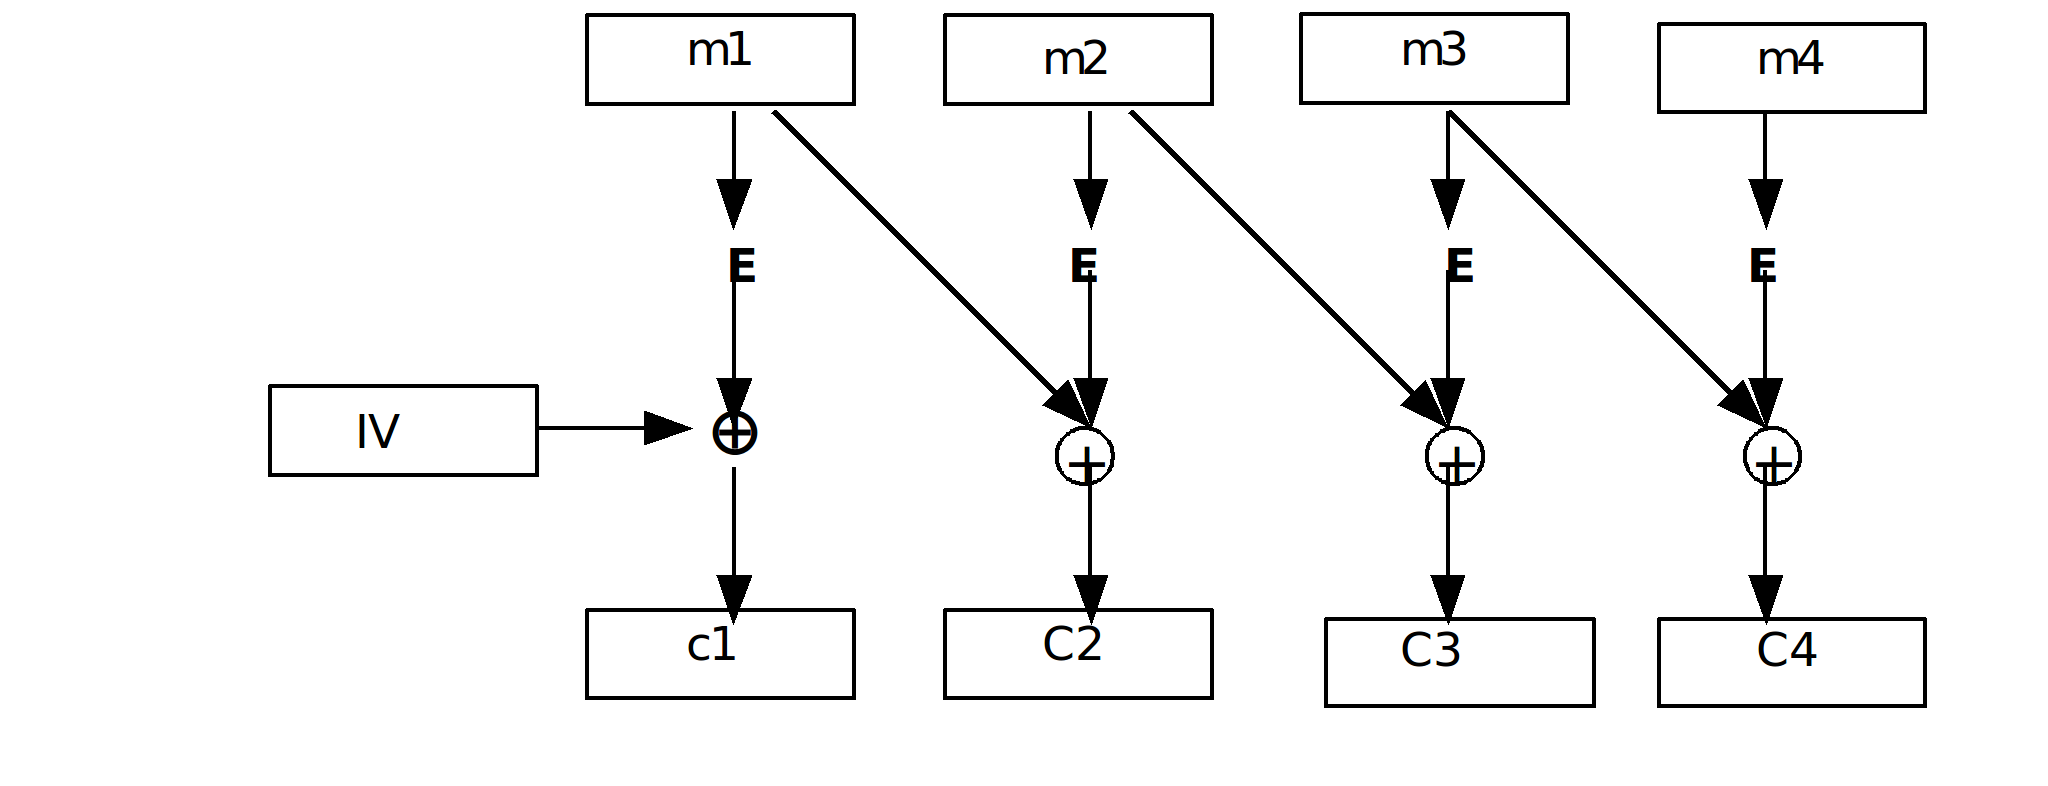
\includegraphics[width=6in]{cbc_variant.png}
\centering
\end{figure}

\vspace{1in}

\section{Multiple Encryption DES [30 pts]}
In answering this question, assume that an average close to $2^{32}$ steps to break an encryption system (find the corresponding key(s)) is tractable, while an average close to $2^{64}$ steps or larger is not. 

\begin{enumerate}
\item Let's assume that you do DES double encryption by encrypting with $k_1$ and doing DES in decrypt mode with $k_2$. Does the same meet-in-the-middle attack described in the textbook work as with double encryption with $k_1$ and $k_2$? If not, how could it be made to work? (Hint: it is possible but requires some tweaks. Please describe your tweaks)

\item Devise a meet-in-the-middle attack to break EDE. That is, find the keys $k_1$ and $k_2$ assuming knowledge of a set of plaintext/ciphertext pairs \textless$m_i, c_i$\textgreater obtained by applying EDE on each $p_i$.  (Hint: you meet either after ED, or before DE)

\item Assume that EDE was deployed using three keys $k_1$ (for step 1 encryption), $k_2$ (for step 2 decryption), and $k_3$ (for step 3 encryption). Is this new version of EDE more secure than the traditional EDE? Explain.

\item Consider the following approach to increase the security of DES. Encryption is done by encrypting the plaintext twice using the same shared secret. Decryption is done by decrypting the ciphertext twice using the same shared secret. Is this approach more secure than the traditional DES?
\end{enumerate}
\vspace{1in}



\section{Breaking Monoaphabetic Cipher Using Frequence Analysis [30 points Bonus. There will be partial credit if you only partially solve it.]}

A monoalphabetic cipher is one where each symbol in the input (called the ``plaintext'') is mapped to a fixed symbol in the output (called the ``ciphertext''). Let's go back to the age where we use statistic analysis (or frequence analysis) to break ciphers (esentially the keys).  It will be a fun assignment, and you can use modern techniques to break old ciphers.

While you can entirely finish this assignment by using pencil and paper, it is more efficient to use (existing) programs. Please \textbf{Find}\footnote{For instance, \url{http://crypto.interactive-maths.com/frequency-analysis-breaking-the-code.html}, which I recommend especially if you don't wanna write code.} or \textbf{write} a program\footnote{Please note that you don't have to write your program in our VM. You can use whatever computing environment convenient to you, e.g., Windows, Linux, Mac, etc., using Java, C, Python, etc.} that reads an input ciphertext, and outputs the (sorted) letter frequencies, diagram (consecutive pairs of letters) frequencies, and trigram (consecutive triplets of letters) frequencies. 

Using this frequence analysis program, decode the following ciphertext. The original plaintext that produced this ciphertext contains only upper case letters;  all punctuation and spaces were removed before encoding.  It was encrypted with a mono-alphabetic cipher.  Explain how you decoded the ciphertext in your answer.

\begin{quote}
\raggedright{
{\tt
WMTLXJAVQNXBTECJIZMWDMEIGXXVTSXRAWHXHTNHVMTVW
KVMXBTECQGXUCXSWXNDXWYNQZQGNQZTIQGPAHRWNRQGVM
XGAVASXJAVJIVMXCTKVTNHPAHRWNRJIVMXCTKVWZWKMVQ
YNQZZMTVVMXSXMTKJXXNWNVMXDQNHADVQGVMXJSWVWKME
WNWKVSIGQSVMXBTKVVZQIXTSKVQPAKVWGIVMQKXMQCXKZ
WVMZMWDMRXNVBXEXNMTLXJXXNCBXTKXHVQKQBTDXVMXEK
XBLXKTNHVMXMQAKXWKWVVMTVWNKWHWQAKKEWBXZWVMZMW
DMQASCXVWVWQNMTKJXXNBTVXBISXDXWLXH
}
}
\end{quote}

\vspace{0.5in}
Reference \url{http://en.wikipedia.org/wiki/Frequency_analysis}
\vspace{0.5in}


\section{Submiting your report}
Please write a report describing how you solve each of the problem above. You can use WORD, or Latex to write the report. The Latex source of this assignement is available at \url{https://www.overleaf.com/read/xfwppdqjbzbt}. Regarding how to use Latex, please see this tutorial if you have 0-experience with it \url{https://www.andy-roberts.net/writing/latex/absolute_beginners}. Please note that latex can be installed in all modern OSes such as Windows, Linux, and Mac.

\end{document}

